% !TeX root = m3talk.tex
% !TeX encoding = UTF-8
% !TeX spellcheck = en_US

\section{discrimination trees}
\subsection{non-linear terms and perfect filtering}

%%% !TeX root = ../m3talk.tex
% !TeX encoding = UTF-8
% !TeX spellcheck = en_US

\begin{frame}
\frametitle{Perfect filtering}
\begin{gather*}
\left\{\begin{array}{lll}
	\TI{1}\mh(\mf(x,x)), &
	\TI{2}\mh(\mg(\ma,x)), &
	\TI{3}\mh(\mf(y,z)), \\
	\TI{4}\mh(\mg(\ma,y)), &
	\TI{5}\mh(\mf(y,x)), &
	\TI{6}\mh(\mg(y,a))
\end{array}\right\}
%%
%		\TI{1}\mh(\mf(x,x)),
%		\TI{2}\mh(\mg(\ma,x)),
%		\TI{3}\mh(\mf(y,z)),
%		\TI{4}\mh(\mg(\ma,y)),
%		\TI{5}\mh(\mf(y,x)),
%		\TI{6}\mh(\mg(y,a))
%%		\\[0.5em]
%
%\ps(t) =
%\begin{cases}
%	* &\text{if $t=x\in\SIGV$} \\
%	\mf.\ps(t_1).\ps(t_2). \cdots.\ps(t_n) &\text{if $t=f(t_1,\ldots,t_n)$}
%	\end{cases}
%
\end{gather*}
%	
\begin{center}
% imperfect filtering	
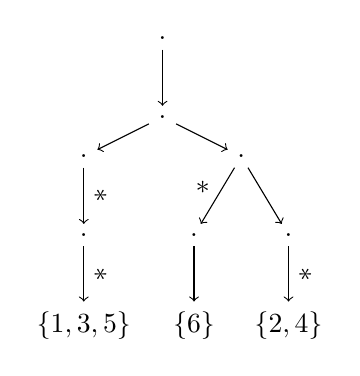
\begin{tikzpicture}[->,sloped,above]

\node[] (root) at (0,0.5) {.};

\node[] (h) at (0,-0.5) {.};
\node[] (f) at (-1,-1)  {.};
\node[] (g) at (1,-1) {.};

\node[] (fx) at (-1,-2) {.};
\node[] (fxx) at (-1,-3.3) {$\{ 1,3,5 \}$ };

\node[] (ga) at (1.6,-2)  {.};
\node[] (gax) at (1.6,-3.3) {$\{ 2,4 \}$};

\node[] (gx) at (.4,-2) {.};
\node[] (gxa) at (.4,-3.3) {$\{ 6 \}$};

\path (root) edge node {$\mh$} (h)

	(h) edge node {$\mf$} (f) 
	edge node {$\mg$}(g)
	
	(f) edge node {$*$} (fx)
	(fx) edge node {$*$} (fxx)
	
	(g) edge node {$\ma$} (ga)
	edge node {$*$} (gx)
		
	(ga) edge node {$*$} (gax)
	(gx) edge node {$\ma$} (gxa)
	
	;
\end{tikzpicture}
%
\hspace{3em}
%
% perfect filtering
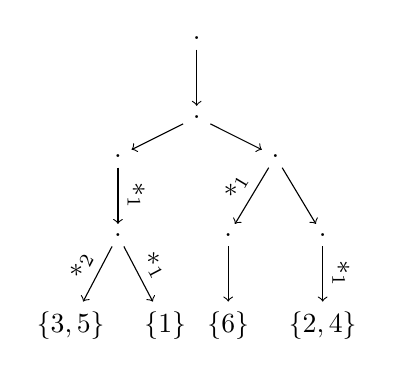
\begin{tikzpicture}[->,sloped,above,node distance=1cm]

\node[] (root) at (0,0.5) {.};

\node[] (h) at (0,-0.5) {.};
\node[] (f) at (-1,-1)  {.};
\node[] (g) at (1,-1) {.};

\node[] (fx) at (-1,-2) {.};
\node[] (fxy) at (-1.6,-3.3) {$\{ 3,5 \}$ };
\node[] (fxx) at (-0.4,-3.3) {$\{ 1 \}$ };

\node[] (ga) at (1.6,-2)  {.};
\node[] (gax) at (1.6,-3.3) {$\{ 2,4 \}$};

\node[] (gx) at (.4,-2) {.};
\node[] (gxa) at (.4,-3.3) {$\{ 6 \}$};

\path (root) edge node {$\mh$} (h)

	(h) edge node {$\mf$} (f) 
	edge node {$\mg$}(g)
	
	(f) edge node {$*_1$} (fx)
	(fx) edge node {$*_1$} (fxx)
	edge node {$*_2$} (fxy)
	
	(g) edge node {$\ma$} (ga)
	edge node {$*_1$} (gx)
		
	(ga) edge node {$*_1$} (gax)
	(gx) edge node {$\ma$} (gxa)
	
	;
\end{tikzpicture}\\[1em]

$\mh(\mf(y,x)) \mapsto \mh.\mf.{*}.{*}$\hspace{6em}$\mh(\mf(y,x)) \mapsto' \mh.\mf.{*_1}.{*_2}$
\end{center}
\end{frame}
%=== example forall ===


%\begin{frame}
%\begin{tikzpicture}
%\node {$\exists $}
%% [clockwise from=-170,sibling angle=-160]
%child {node {$[a,b,c]$}}
%child {node {${\mathsf p}$}
%% [clockwise from=-90,sibling angle=0]
% child {node {$a$}}};
%     \end{tikzpicture}
%     
%$(\exists [a,b,c]:({\mathsf p}(a)))$
%\end{frame}

\begin{frame}
	\frametitle{Non-linear terms}
	\def\dw{1}
	\def\dh{1}
	\begin{exampleblock}{}
	\begin{minipage}{4.5cm}
		
	\begin{tikzpicture}[->,right]
	
	\node (root) at (1.2,0) {.};
	\node (f) at (1.2,-1) {.};
	\node (fh) at (0.2,-2) {.};
	\node (fha) at (0.25,-3) {.};
	\node (fhaa) at (-1,-4) {1};
	\node (fhah) at (1,-4) {.};
	\node (fhaha) at (1,-5) {2};
	
	\node (fx) at (2.2,-2) {.};
	\node (fxy) at (2.2,-3) {3};
	
	\path 
		(root) 
			edge[colHi] node {$\mf$} (f)
		(f) edge[sloped,above] node {$\mh$} (fh)
			edge[sloped,above,colHi] node {${*}$} (fx)
			edge[bend left,dashed,left,colHi] (fha)
		(fh) edge node {$\ma$} (fha)
		
			
		(fha) edge[sloped,above] node {$\ma$} (fhaa)
		 edge[sloped,above] node {$\mh$} (fhah)
		 edge[bend left,dashed,right,colLo] (fhaa) 
		 edge[bend right,dashed,left,colHi]  (fhaha) 
		 
		 (fhah) edge node {$\ma$} (fhaha)
		 
		 (fx) edge[colHi]  node {${*}$} (fxy)
		;

	\end{tikzpicture}
	
	\end{minipage}
	\begin{minipage}{7cm}
		$
		\{\TI{1}\mf(\mh(\ma),\ma), 
		\TI{2}\mf(\mh(\ma),\mh(\ma))\},
		\TI{3}\mf(x,y) \}
		$\\[0.7em]
		
	The  terms $\mf(x,y)$ and $\mf(z,z)$\\ 
	share the preorder-term $\mf{*}{*}$.\\[0.7em]
	But $\mf(\mh(\ma),\ma)$ is not an instance of $\mf(z,z)$.
\end{minipage}
\end{exampleblock}
	\end{frame}

\begin{frame}
${\mathsf f}({\mathsf a},x)$

\begin{tikzpicture}
\node {${\mathsf f}$}
child {node {${\mathsf a}$}}
child {node {$x$}};
 \end{tikzpicture}

${\mathsf f}({\mathsf a},x)\approx {\mathsf f}(x,{\mathsf a})$

\begin{tikzpicture}
\node {$\approx $}
% [clockwise from=-150,sibling angle=-120]
child {node at (-0.7,1) {${\mathsf f}$}
 [clockwise from=-130,sibling angle=-80]
 child {node {${\mathsf a}$}}
 child {node {$x$}}}
child {node at (0.7,1){${\mathsf f}$}
 [clockwise from=-130,sibling angle=-80]
 child {node {$x$}}
 child {node {${\mathsf a}$}}};
 \end{tikzpicture}
\end{frame}